\chapter{Design}
Det er i projektet arbejdet lodret ned igennem lagene når nye features skulle designes. Systemmet er udviklet så featuren fuldstændigt ned igennem lagene. Det er derfor valgt at beskrive en feature hele vejen ned igennem for at eksemplificere selve designet af systemmet. For fuld beskrivelse af systemmetdesignet se dokumentationen. 

\section{Modeldesign}

Ud fra domæneanalysen er dataen der giver mening at persistere fundet, og på fig. \ref{fig:BarteradModel} A) kan ses hvad der ud fra analysen skulle gemmes i forbindelse med barterads.

\begin{figure}[H]
	\centering
	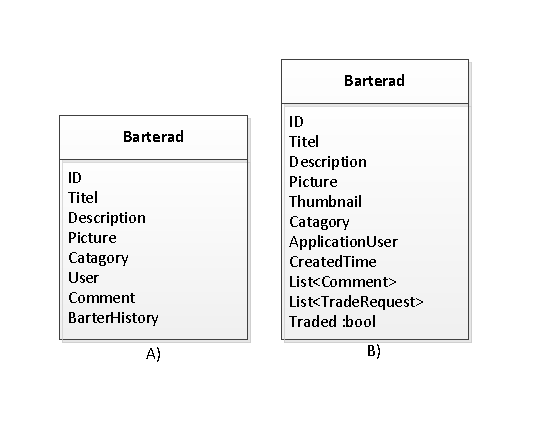
\includegraphics
	[width=140mm]{figures/BarterAdModels.pdf}
	\caption{A) BarterAd model fra domæneanalyse  B) Aktuel model}
	\label{fig:BarteradModel}
\end{figure} 

Efter arbejde, og iterationer igennem den agile arbejdsmetode er der udfærdiget et endeligt modeldesign af barterads som kan ses på \ref{fig:BarteradModel} B.  
I designetfasen bliver det bestemt hvilke sikkerhedskriterier data i databasen skal overholdeholde. Til dette konkrete eksempel kan der en række krav til modellen som skal være opfyldt. Disse ses her:

\begin{itemize}
	\item Barterads skal være tilknyttet en ApplicationUser
	\item Barterads skal have et oprettelsestidspunkt, men dette laves her
	\item Barterads må have en maksiaml beskrivelseslængde på 500 tegn
\end{itemize}

Modellen opretter igennem EF databasestrukturen og til derefter at tilgå de data anvendes det tidligere nævnte repository pattern som standardisere måden at tilgå data på.

Selve funktionaliteten af hvad der sker når klienten skal oprette en barterad, sker igennem serverens controller. 

\section{Controller}  

Klienten tilgår controlleren igennem en URL, og i controllerne ligger funktionalitet af BargainBarter systemmet. Det er controllernes opgave at opdatere det view som brugeren ser, samt styre kommunikationen mellem viewet og modellen. På fig \ref{fig:SDOpretBarterAd} ses en forsimplet udgave af hvad der sker når under oprettelsen af et Barterad. \\
 
\noindent Som det det ses på figur \ref{fig:SDOpretBarterAd} trykker brugeren ind for at lave en ny annonce. Systemmet registrerer at der er trykket på en knap, og kalder den til viewelementet tilhørende action, der returnere til create barterad view. I dette view kan der indtastes data til barterads. Brugeren indtaster data og submitter. Controlleren opretter så selve barteraden og tilføjer de systemgenererede data. Disse inkludere tilhørsbrugeren og oprettelsestidspunkt. I controlleren sørges for at brugeren skal være logget ind, for at kunne oprette annonce. Desuden skal alle felter være udfyldt i oprettelsen, hvilken er sikret både i viewet og modellen.     


\begin{figure}[H]
	\centering
	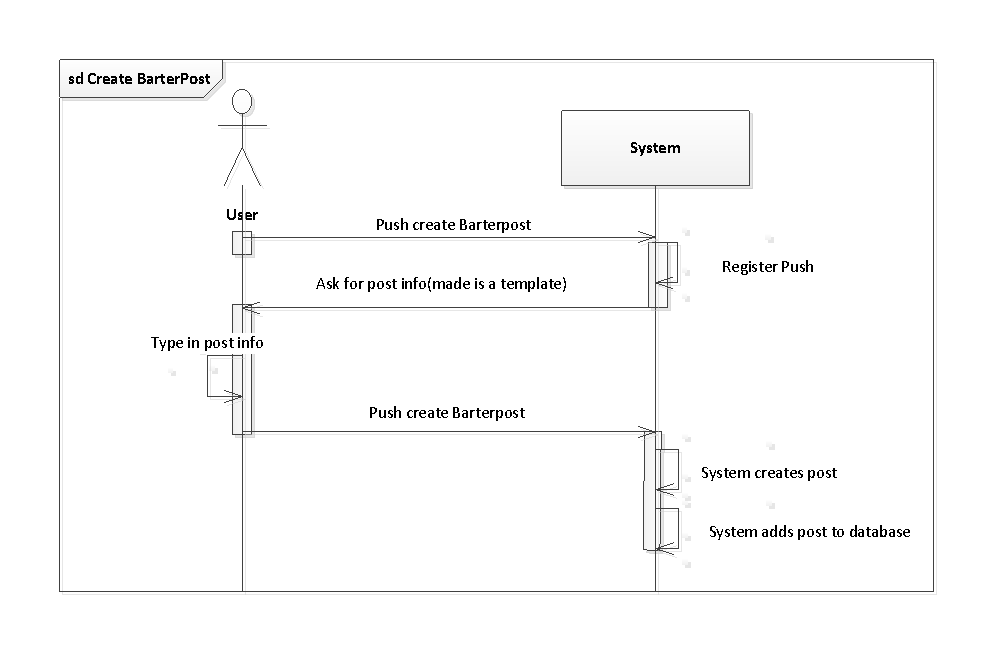
\includegraphics
	[width=140mm]{../Dokumentation/figures/SDOpretBytteAnnonce.PDF}
	\caption{Sekvensdiagram for, hvordan en barterAd bliver fundet i DB}
	\label{fig:SDOpretBarterAd}
\end{figure}

På fig. \ref{SDOpretBarterAd} ses et forsimplet sekvensdiagram af annonceoprettelsen. 

\section{View} 

\section{BLL}

\section{DAL}